\subsubsection{Mediciones con imágenes}

Para poder corregir la trayectoria del robot de forma dinámica, es decir interfiriendo cual va a ser el vector de movimiento, cuando este se encuentra realizando un recorrido es necesario tener un conocimiento del entorno en el cual se va a mover. El beneficio que trae esta incorporación es poder aumentar la precisión de los movimientos que va a realizar cuando el robot ejecuta un trayecto, en realidad, la denominación correcta sería poder disminuir el error de la trayectoria a efectuar.

Esta medición y corrección en tiempo real se suma a las iteraciones de ajuste de trayectoria mediante la medición de imanes por sensores hall y filtro de Kalman, estas iteraciones por supuesto mejoran el movimiento que efectúa el robot pero también siempre es importante tratar de disminuir el error los mas posible ya que sin ningún tipo de medición sobre el entorno y los movimientos, el único parámetro medible es la distancia recorrida por las ruedas, y como sabemos esto no es suficiente para determinar con precisión la ubicación del robot.

El reconocimiento del entorno de desplazamiento del robot se puede realizar de muchas maneras, desde sensores ultrasónicos hasta cámaras fotográficas, y por supuesto dependiendo cual se selecciona la precisión de la medición va a aumentar o disminuir.
En base a los modelos anteriores del robot que usaron sensores de ultrasonido para determinar la distancia de los objetos que se encuentran en frente del robot, notamos que la precisión de los mismos no nos es suficiente para influir de manera conveniente en la trayectoria. Es por ello que decidimos usar como alternativa una cámara fotográfica, y por ende el procesamiento de imágenes para identificar los elementos que creamos necesarios dentro de la foto para determinar qué información podemos extraer de ahí, cómo interpretarla y finalmente influir en el comportamiento del robot.

El microcontrolador ESP-32 cuenta con un modelo que incorpora la posibilidad de añadirle un cámara de manera extraíble, desafortunadamente no es el mismo modelo el cual maneja la lógica del comportamiento del robot por lo cual fue necesario la incorporación de un nuevo microcontrolador y sumarle un sostén por encima del robot para que este sostenga la cámara y podamos obtener imágenes de manera más cómoda.

\begin{figure}[H]
   \centering
   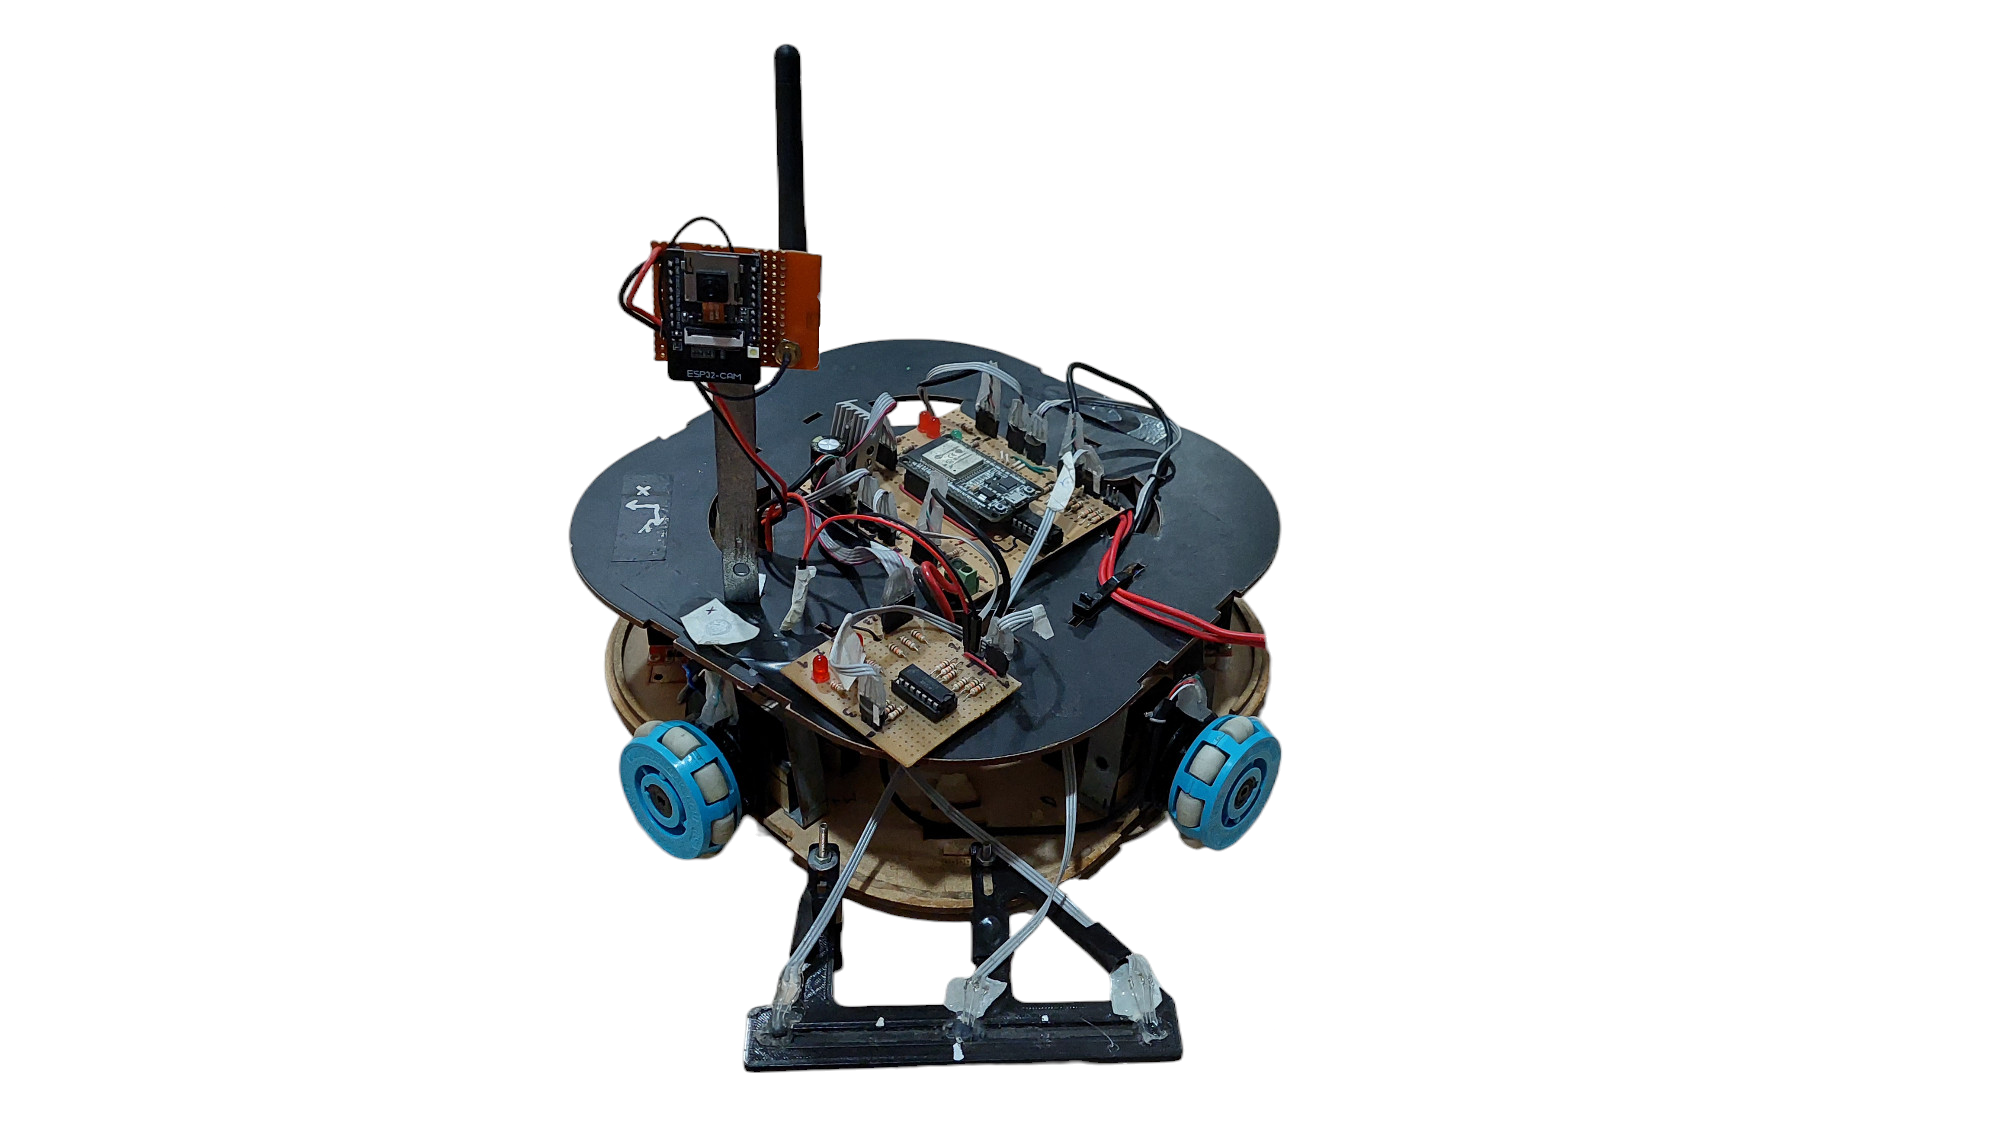
\includegraphics[width=1.0\linewidth]{images/robot_camara.png}
   \caption{Robot con la ESP32-CAM incorporada}
   \label{fig:robot_camara}
\end{figure}

Con el solo hecho de tomar una fotografía con el microcontrolador, usamos la mayor de su procesamiento en esa tarea. Realizando distintas pruebas con las resoluciones de imágenes que la cámara pone a disposición nos dimos cuenta que hasta es necesario añadirle un opción para habilitar una memoria RAM externa para almacenar las imágenes. Esto nos sirvió para darnos cuenta que no íbamos a poder realizar el procesamiento de las imágenes dentro del microcontrolador y lo mejor sería seguir acoplado al paradigma de IoT el cual nos plantea que este dispositivo solo va a servir para tomar la fotografía y enviarla a otro servidor el cual se va a encargar de procesar la imagen.